% Deixar três (3) linhas em branco antes dos títulos de cápitulos
% %%%%%%%%%%%%%%%%%%%%%%%%%%%%%%%%%%%%%%%%%%%%%%%%%%%%%%%%%%%%%%%%%%%%%%%%%%
\section{INTRODUÇÃO}
% %%%%%%%%%%%%%%%%%%%%%%%%%%%%%%%%%%%%%%%%%%%%%%%%%%%%%%%%%%%%%%%%%%%%%%%%%%
% Deixar uma (1) linha em branco após cada título

A introdução deve apresentar o contexto do estágio, sua importância e um panorama geral do que será abordado no relatório.


% Deixar três (2) linhas em branco antes dos títulos das seções
% -------------------------------------------------------------------------
\subsection{Área de Conhecimento} \label{sec:areaconhecimento}
% -------------------------------------------------------------------------
% Deixar uma (1) linha em branco após o título da seção, para separar do texto
Explicação sobre a relevância do estudo, destacando sua importância acadêmica, científica ou prática.


% -------------------------------------------------------------------------
\subsection{Objetivo Geral} \label{sec:objetivo-geral}
% -------------------------------------------------------------------------

Descrição do propósito central do estudo.


% -------------------------------------------------------------------------
\subsection{Objetivos Específicos} \label{sec:objetivos-especificos}
% -------------------------------------------------------------------------
Lista de metas detalhadas que, quando atingidas, contribuem para o objetivo geral. 


Exemplo:
\begin{alineas} % {enumerate} -> para números, {alineas} -> para letras
    \item Analisar e inferir ...
    
    \item Modelar e implementar uma ...
    
    \item Realizar análise e implementação do ...
    
    \item Desenvolvimento de um ...
\end{alineas}


% -------------------------------------------------------------------------
\subsection{Justificativa} \label{sec:justificativa}
% -------------------------------------------------------------------------

Definição clara do que o trabalho pretende alcançar, e a relevância do estágio para sua formação.

% %%%%%%%%%%%%%%%%%%%%%%%%%%%%%%%%%%%%%%%%%%%%%%%%%%%%%%%%%%%%%%%%%%%%%%%%%%
\section{APRESENTAÇÃO DA EMPRESA} \label{ch:apresentacao-empresa}
% %%%%%%%%%%%%%%%%%%%%%%%%%%%%%%%%%%%%%%%%%%%%%%%%%%%%%%%%%%%%%%%%%%%%%%%%%%
Forneça um um paragrafo introdutorio, sobre o que será apresentado nesse seção, exemplo nome da empresa e aspectos que serão apresentados sobre a empresa.

% -------------------------------------------------------------------------
\subsection{``nome da empresa''} \label{sec:nome-da-empresa}
% -------------------------------------------------------------------------
Forneça uma visão geral da empresa onde o estágio foi realizado, incluindo sua história, missão, valores, estrutura organizacional e principais atividades


% %%%%%%%%%%%%%%%%%%%%%%%%%%%%%%%%%%%%%%%%%%%%%%%%%%%%%%%%%%%%%%%%%%%%%%%%%%
\section{METODOLOGIA} \label{ch:metodologia}
% %%%%%%%%%%%%%%%%%%%%%%%%%%%%%%%%%%%%%%%%%%%%%%%%%%%%%%%%%%%%%%%%%%%%%%%%%%

Descreva como o estágio foi conduzido, incluindo métodos de trabalho, ferramentas utilizadas e estratégias para o aprendizado.

\subsection{Cronograma} \label{sec:cronograma}

% -------------------------------------------------------------------------
presente um cronograma das atividades desenvolvidas ao longo do estágio, especificando períodos e tarefas realizadas.


% %%%%%%%%%%%%%%%%%%%%%%%%%%%%%%%%%%%%%%%%%%%%%%%%%%%%%%%%%%%%%%%%%%%%%%%%%%
\section{REVISÃO BIBLIOGRÁFICA} \label{ch:referencial-teorico}
% %%%%%%%%%%%%%%%%%%%%%%%%%%%%%%%%%%%%%%%%%%%%%%%%%%%%%%%%%%%%%%%%%%%%%%%%%%

Forneça um parágrafo introdutório com o objetivo de introduzir o que será apresentado nesta seção. Na sequencia crie as subseções necessárias para manter a seção organizada. 

Neste capítulo deve ser apresentado uma revisão da literatura sobre o tema do trabalho, apresentando conceitos, teorias e estudos relevantes que fundamentam o trabalho desenvolvido.  


\begin{figure} [htb]
    \begin{center}
	 \caption{\label{fig:ag}Esquema de um algoritmo genético}
        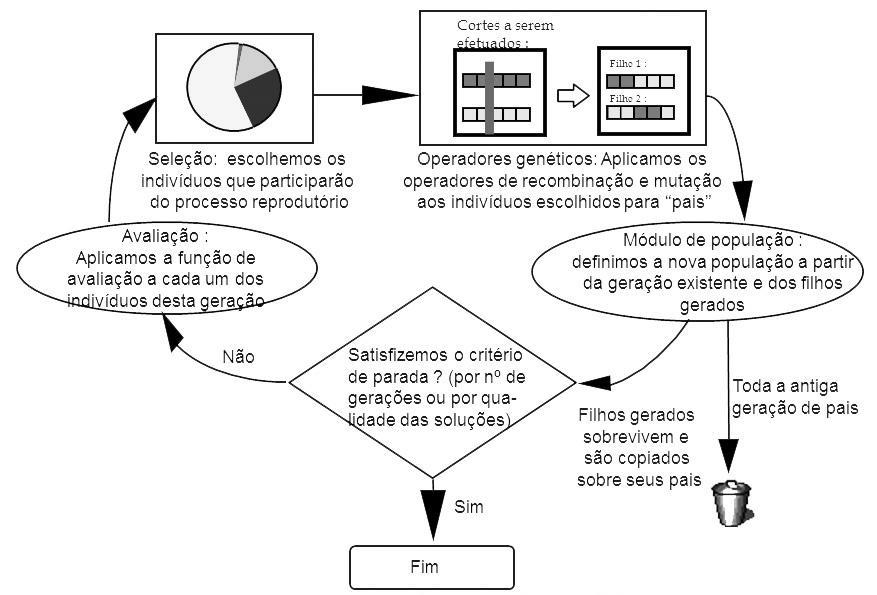
\includegraphics[scale=0.6]{imagens/revisao-bibliografica/esquemaAlgGenetico_pag64.png}
	\legend{Fonte: \citeonline[p. 64]{linden2012}.}
    	\end{center}
    \end{figure}
    
Incluindo uma figura de autoria própria.
\begin{figure} [htb]
\begin{center}
	 \caption{\label{fig:ambiente}Ambiente abordado}
	    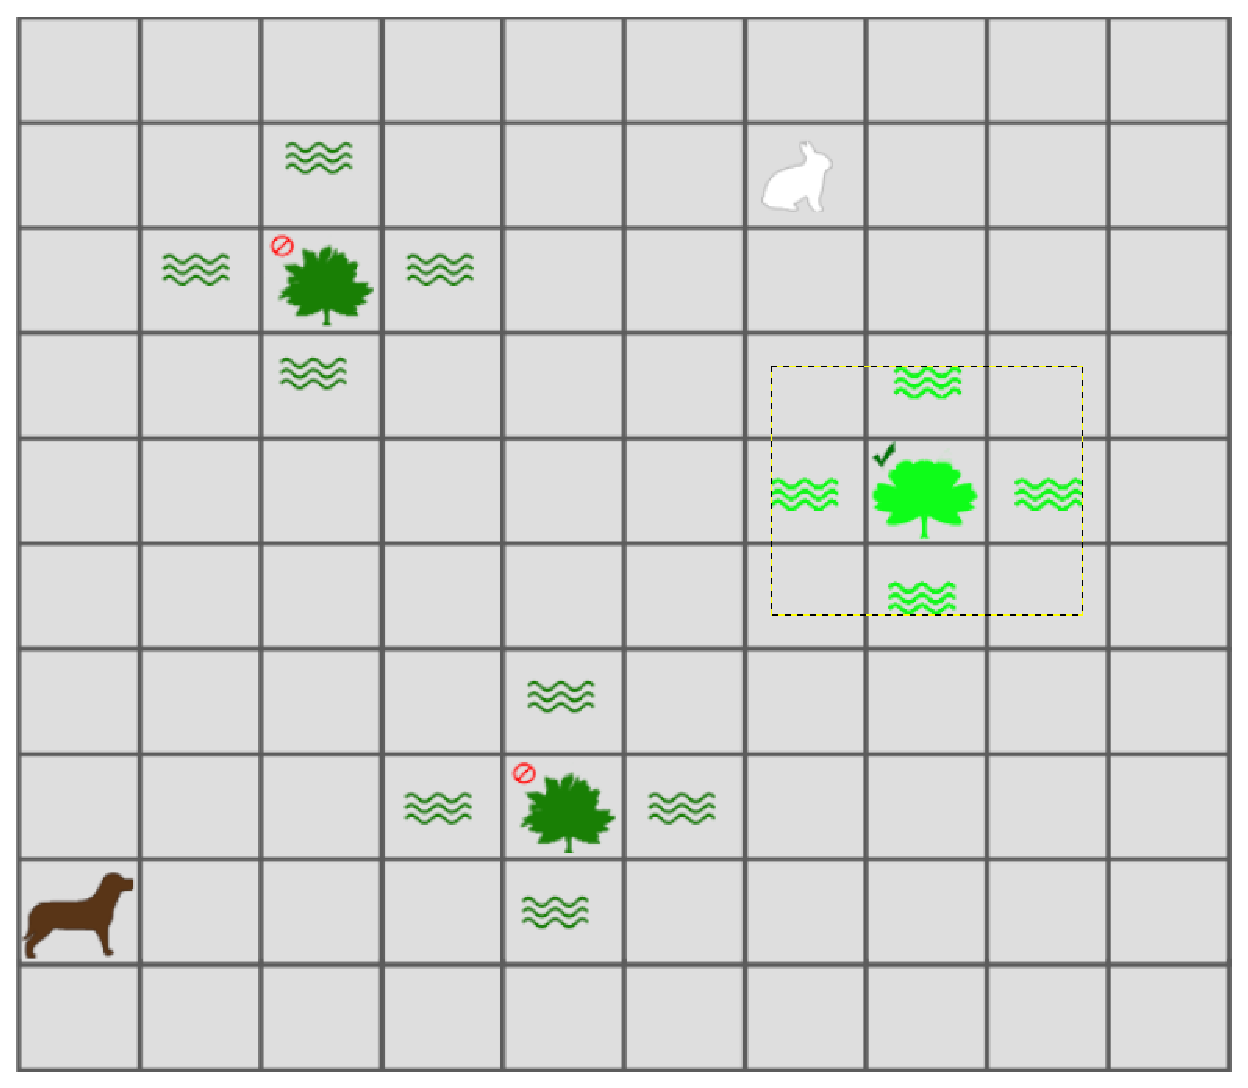
\includegraphics[scale=0.3]{imagens/revisao-bibliografica/ambiente.eps}
	\legend{Fonte: autoria própria.}
    \end{center}
\end{figure}

\subsection{tema 1 relacionado ao trabalho}



\subsection{tema 2 relacionado ao trabalho}


Exemplo 1 de citação, \cite{almeida2022}

Exemplo 2 de citação, \citeonline{almeida2022}\\ \\
% Deixar duas (2) linhas em branco antes do o título de uma seção
Lista com citações de  diferentes tipos de documentos, para gerar o exemplo de\\ \textbf{Referências} ao final do documento.\\ \\
Dissertação, \cite{almeida2022}\\
Trabalho publicado em Conferência, \cite{cbsoft2023}\\
Página web, \cite{ferreira2020}\\
Manual, \cite{latex2023}\\
Capitulo de livro, \cite{mendes2019}\\
Relatório técnico, \cite{oliveira2020}\\
Livro, \cite{linden2012}\\
Tese de doutorado, \cite{rodrigues2021}\\
Artigo científico, \cite{silva2023}\\
Livro de Conferência, \cite{souza2022}


% %%%%%%%%%%%%%%%%%%%%%%%%%%%%%%%%%%%%%%%%%%%%%%%%%%%%%%%%%%%%%%%%%%%%%%%%%%
\section{ATIVIDADES DESENVOLVIDAS} \label{ch:atividades-desenvolvidas}
% %%%%%%%%%%%%%%%%%%%%%%%%%%%%%%%%%%%%%%%%%%%%%%%%%%%%%%%%%%%%%%%%%%%%%%%%%%
Descreva em detalhes todas as atividades realizadas no estágio, explicando sua importância e os desafios enfrentados.

Crie subseções para dividir as diferentes atividades e etapas  envolvidas no estágio.

% -------------------------------------------------------------------------
\subsection{ Seção Atividade Parcial 1} \label{sec:definir-tituto-da-secao1}
% -------------------------------------------------------------------------

Discussão detalhada de um dos tópicos fundamentais para o entendimento do problema abordado. \\ Caso necessário, pode ser criado subseções

Para referenciar a tabela você pode usar o comando "autoref" ex: \autoref{tab:resultados1}, ou o "ref", ex: \ref{tab:resultados1}

\begin{table}[htb]
\centering
\caption{Exemplo de tabela conforme a ABNT}
\label{tab:resultados1}
\begin{tabular}{p{0.3\textwidth} p{0.3\textwidth} p{0.3\textwidth}} % Ajuste das larguras das colunas
    \hline
    \textbf{Coluna 1} & \textbf{Coluna 2} & \textbf{Coluna 3} \\
    \hline
    Informação 1 & Informação 2 & Informação 3 \\
    Informação 4 & Informação 5 & Informação 6 \\
    Informação 7 & Informação 8 & Informação 9 \\  
    \hline
\end{tabular}
\legend{Fonte: autoria própria.}
\end{table}

\begin{table}[htb]
\centering
\caption{Exemplo de tabela conforme a ABNT}
\label{tab:resultados2}
\begin{tabular}{>{\centering\arraybackslash}p{0.3\textwidth}  >{\centering\arraybackslash}p{0.3\textwidth}  >{\centering\arraybackslash}p{0.3\textwidth}} % Ajuste das larguras das colunas
    \hline
    \textbf{Coluna 1} & \textbf{Coluna 2} & \textbf{Coluna 3} \\
    \hline
    Informação 1 & Informação 2 & Informação 3 \\
    Informação 4 & Informação 5 & Informação 6 \\
    Informação 7 & Informação 8 & Informação 9 \\  
    \hline
\end{tabular}
\legend{Fonte: autoria própria.}
\end{table}


\begin{table}[ht]
    \centering
    \caption{Exemplo de tabela conforme a ABNT}
    \label{quad:exemplo}
    \begin{tabular}{p{3cm} p{4cm} p{3cm}}
        \hline%\toprule
        \textbf{Coluna 1} & \textbf{Coluna 2} & \textbf{Coluna 3} \\
        \hline%\midrule
        Informação 1 & Informação 2 & Informação 3 \\
        Informação 4 & Informação 5 & Informação 6 \\
        Informação 7 & Informação 8 & Informação 9 \\
        \hline%\bottomrule
    \end{tabular}
    \legend{Fonte: \citeonline{linden2012}.}
\end{table}



% -------------------------------------------------------------------------
\subsection{ Seção Atividade Parcial 2} \label{sec:definir-tituto-da-secao2}
% -------------------------------------------------------------------------

Discussão detalhada de um dos tópicos fundamentais para o entendimento do problema abordado. \\ Caso necessário, pode ser criado subseções


% %%%%%%%%%%%%%%%%%%%%%%%%%%%%%%%%%%%%%%%%%%%%%%%%%%%%%%%%%%%%%%%%%%%%%%%%%%
\section{Considerações Finais} \label{ch:consideracoes-finais}
% %%%%%%%%%%%%%%%%%%%%%%%%%%%%%%%%%%%%%%%%%%%%%%%%%%%%%%%%%%%%%%%%%%%%%%%%%%
Resuma as principais contribuições do trabalho, avalie o cumprimento dos objetivos definidos na seção \textbf{Objetivos} e sugira possíveis direções para trabalhos futuros.\\
Além disso, reflita sobre a experiência do estágio, destacando os principais aprendizados, os desafios superados e o impacto na sua formação. 